\documentclass{ctexart}
\usepackage{amsmath}
\usepackage{graphicx,booktabs,array}

\title{方程求解}
\author{St Maxwell}
\begin{document}
\maketitle

问题:求方程 $f(x) = x^2 + x - 0.39 = 0 $ 的根。

\begin{figure}[htbp]
  \centering
  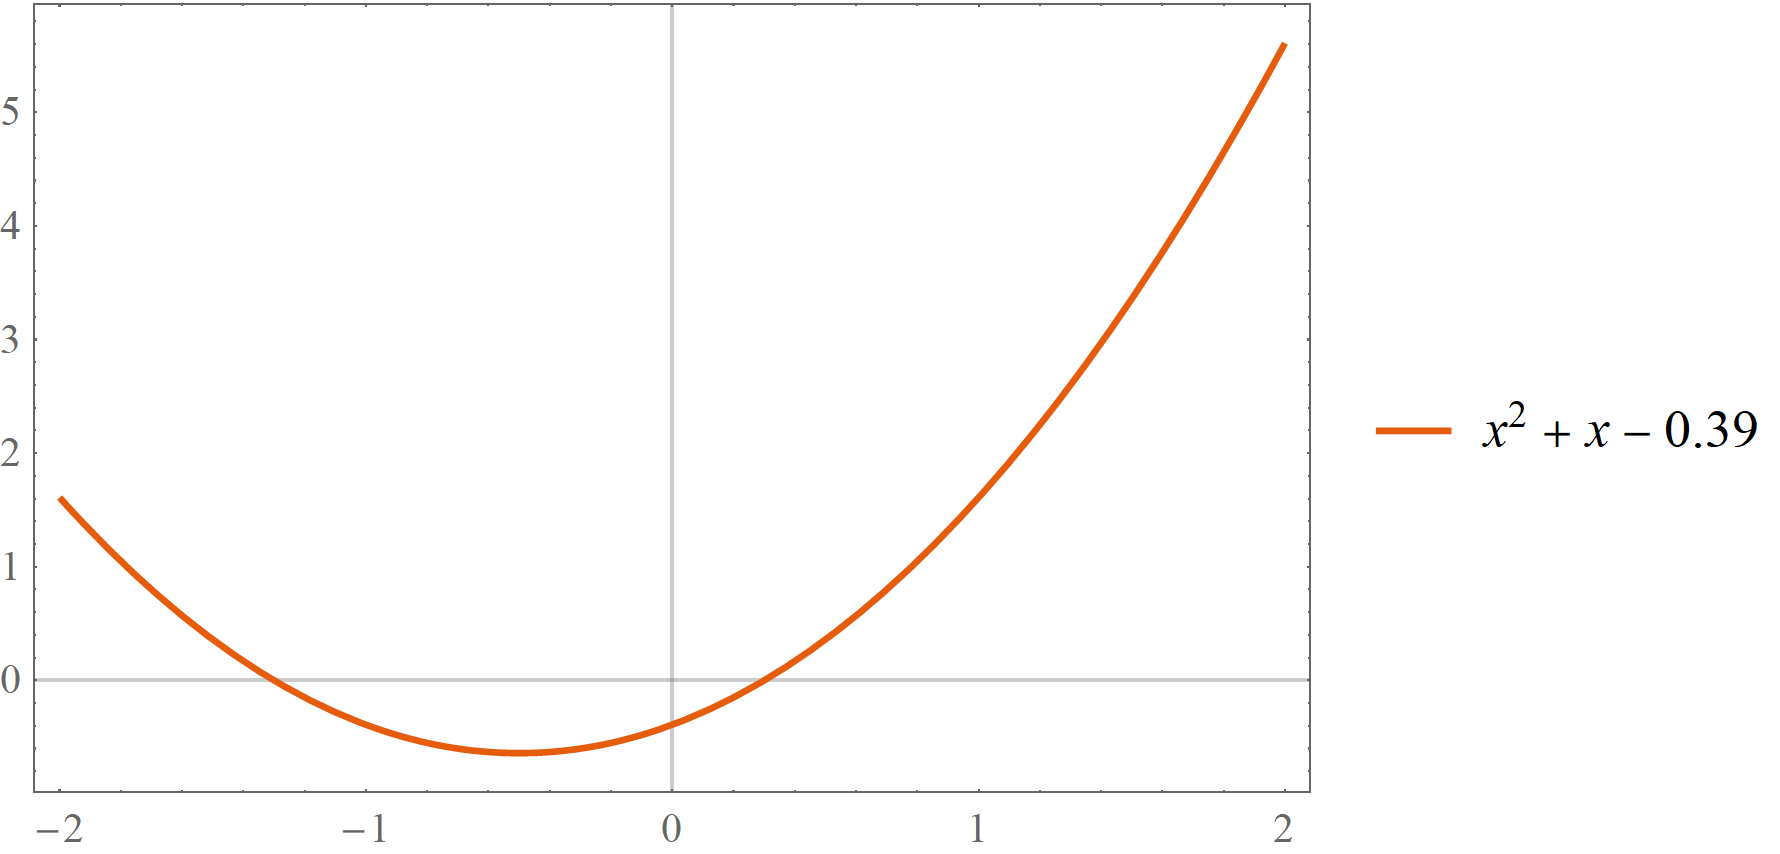
\includegraphics[width=30em]{plot1.png}
  \caption{$f(x)$}
  \label{fig:plot1}
\end{figure}

上图为$f(x)$,方程$f(x) = x^2 + x - 0.39 = 0 $的两个根分别为$0.3$和$-1.3$。

\section{二分法}

对于两个根,我们分别取$[0,1]$和$[-2,-1]$作为初猜的区间。假定结果精确到小数点后6位(其余方法也是如此),所需步数可计算得到:
\[
|x_c - r| < \frac{1}{2^{(n+1)}} < 0.5\times10^{-6}
\]
得到
\[
n > \frac{7}{\lg{2}} \approx 19.9 = 20
\]
因此进行20次二分便可达到精度要求。下面以右侧的根求解为例:

\begin{table}[htpb]
\centering
\caption{二分法迭代过程}
$\begin{array}{cccc}
    \toprule
    n & a_n & c_n & b_n \\
    \midrule
     1 & 0.0000000 & 0.5000000 & 1.0000000 \\
     2 & 0.0000000 & 0.2500000 & 0.5000000 \\
     3 & 0.2500000 & 0.3750000 & 0.5000000 \\
     4 & 0.2500000 & 0.3125000 & 0.3750000 \\
     5 & 0.2500000 & 0.2812500 & 0.3125000 \\
     6 & 0.2812500 & 0.2968750 & 0.3125000 \\
     7 & 0.2968750 & 0.3046875 & 0.3125000 \\
     8 & 0.2968750 & 0.3007812 & 0.3046875 \\
     9 & 0.2968750 & 0.2988281 & 0.3007812 \\
    10 & 0.2988281 & 0.2998047 & 0.3007812 \\
    11 & 0.2998047 & 0.3002930 & 0.3007812 \\
    12 & 0.2998047 & 0.3000488 & 0.3002930 \\
    13 & 0.2998047 & 0.2999268 & 0.3000488 \\
    14 & 0.2999268 & 0.2999878 & 0.3000488 \\
    15 & 0.2999878 & 0.3000183 & 0.3000488 \\
    16 & 0.2999878 & 0.3000031 & 0.3000183 \\
    17 & 0.2999878 & 0.2999954 & 0.3000031 \\
    18 & 0.2999954 & 0.2999992 & 0.3000031 \\
    19 & 0.2999992 & 0.3000011 & 0.3000031 \\
    20 & 0.2999992 & 0.3000002 & 0.3000011 \\
    \bottomrule
\end{array}\label{table:bisect}$
\end{table}

如表\ref{table:bisect}所示,函数的解在$(0.2999992,0.3000011)$之间,区间中点$c_{20}=0.3000002$为最佳估计值。

\section{不动点迭代}

首先可以简单地将方程改写为:
\[
x = 0.39 - x^2 = g_1(x)
\]
由此可以构造不动点迭代函数$g_1(x)$,其图像见图\ref{fig:plot2}。

\begin{figure}[htbp]
  \centering
  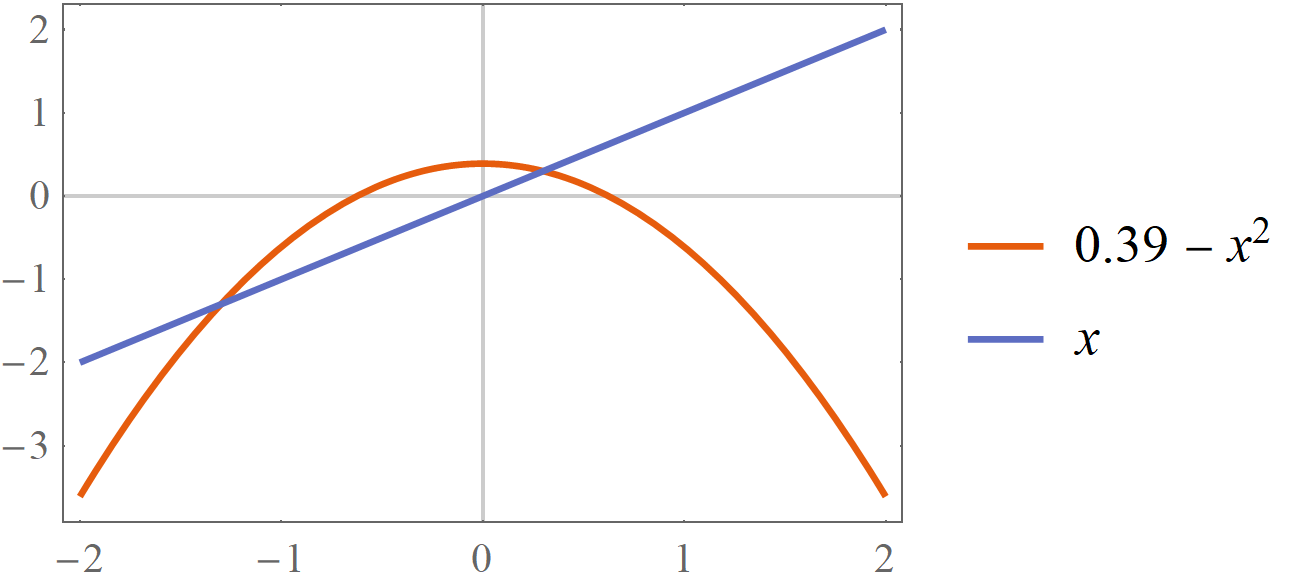
\includegraphics[width=30em]{plot2.png}
  \caption{$g_1(x)$}
  \label{fig:plot2}
\end{figure}

可以看出函数应当有两个不动点,即对应方程的两个解。但并非每个在不动点附近进行不动点迭代都能够收敛:
\[
g'_1(x) = -2x
\]
\[
|g'_1(0.3)| = 0.6 < 1,\quad |g'_1(-1.3)| = 2.6 > 1
\]
因此仅有右边的不动点进行不动点迭代可收敛,而且由于迭代速度$S=0.6>0.5$,表明收敛速度小于二分法。

\begin{table}[htpb]
\centering
\caption{不动点迭代过程}
$\begin{array}{ccc}
    \toprule
n & x_n & g_1(x_n) \\
\midrule
 1 & 0.5000000 & 0.1400000 \\
 2 & 0.1400000 & 0.3704000 \\
 3 & 0.3704000 & 0.2528038 \\
 4 & 0.2528038 & 0.3260902 \\
\multicolumn{3}{c}{\vdots} \\
25 & 0.3000010 & 0.2999994 \\
26 & 0.2999994 & 0.3000004 \\
27 & 0.3000004 & 0.2999998 \\
28 & 0.2999998 & 0.3000001 \\
    \bottomrule
\end{array}\label{table:fpi1}$
\end{table}

可以看到,不动点迭代经过28步才收敛。

所以我们需要考虑构造更好的不动点迭代函数:
\[
g_2(x) = \frac{0.39}{x + 1},\quad g_3(x) = \frac{0.39 - x}{x}
\]

$g_2(x)$和$g_3(x)$函数图像

\begin{figure}[htbp]
  \centering
  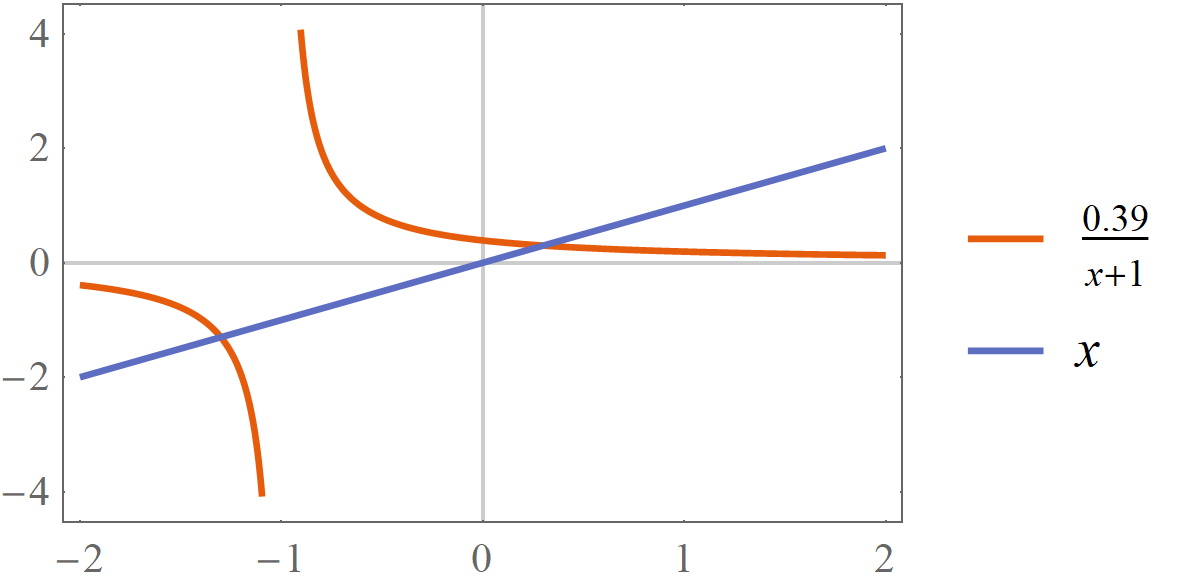
\includegraphics[width=16em]{plot3.png}
  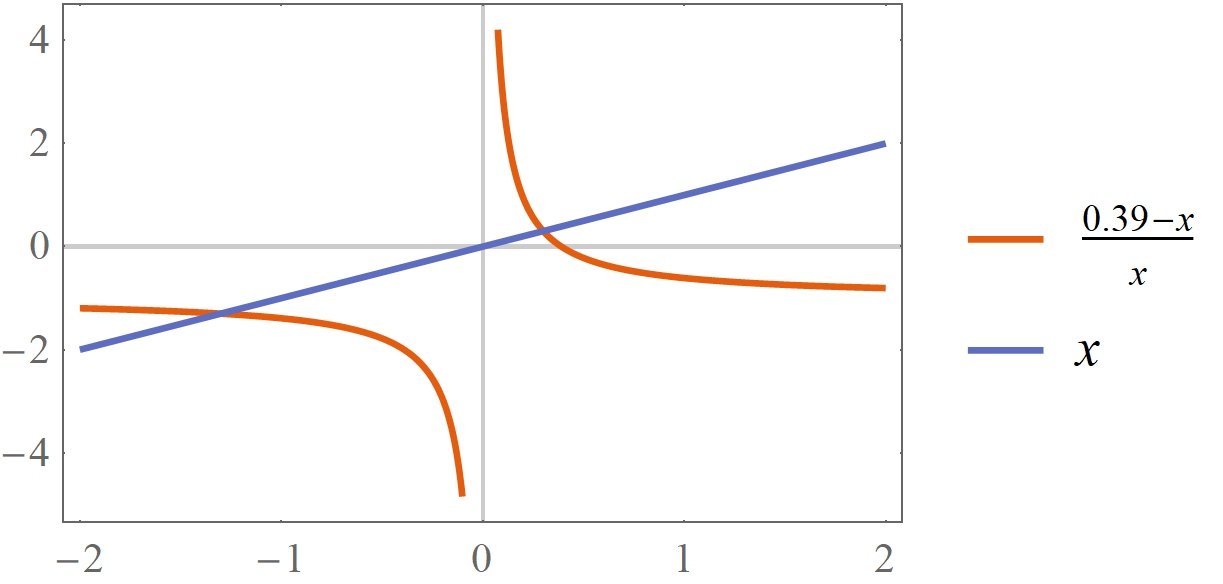
\includegraphics[width=16em]{plot4.png}
  \caption{$g_2(x)$和$g_3(x)$}
  \label{fig:plot3}
\end{figure}

\[
|g'_2(0.3)| = 0.23 < 1,\quad |g'_2(-1.3)| = 4.33 > 1
\]
\[
|g'_3(0.3)| = 4.33 > 1,\quad |g'_3(-1.3)| = 0.23 < 1
\]
虽然我们构造的两个新函数同样无法同时用于得到两个根,但对于可收敛的不动点而言,其收敛速度将会更快。

\begin{table}[htpb]
\centering
\caption{不动点迭代过程}
$\begin{array}{ccccc}
    \toprule
n & x_n & g_2(x_n) & x'_n & g_3(x'_n) \\
\midrule
 1 & 0.5000000 & 0.2600000 & -1.5000000 & -1.2600000 \\
 2 & 0.2600000 & 0.3095238 & -1.2600000 & -1.3095238 \\
 3 & 0.3095238 & 0.2978182 & -1.3095238 & -1.2978182 \\
 4 & 0.2978182 & 0.3005043 & -1.2978182 & -1.3005043 \\
 5 & 0.3005043 & 0.2998837 & -1.3005043 & -1.2998837 \\
 6 & 0.2998837 & 0.3000269 & -1.2998837 & -1.3000269 \\
 7 & 0.3000269 & 0.2999938 & -1.3000269 & -1.2999938 \\
 8 & 0.2999938 & 0.3000014 & -1.2999938 & -1.3000014 \\
 9 & 0.3000014 & 0.2999997 & -1.3000014 & -1.2999997 \\
10 & 0.2999997 & 0.3000001 & -1.2999997 & -1.3000001 \\
    \bottomrule
\end{array}\label{table:fpi2}$
\end{table}

这两个新的函数均只用了10步便收敛成功,比二分法的速度更快。

\section{Newton法}
Newton法的迭代公式为:
\[
x_{i+1} = x_i - \frac{f(x_i)}{f'(x_i)}
\]

其示意图如下:

\begin{figure}[htbp]
  \centering
  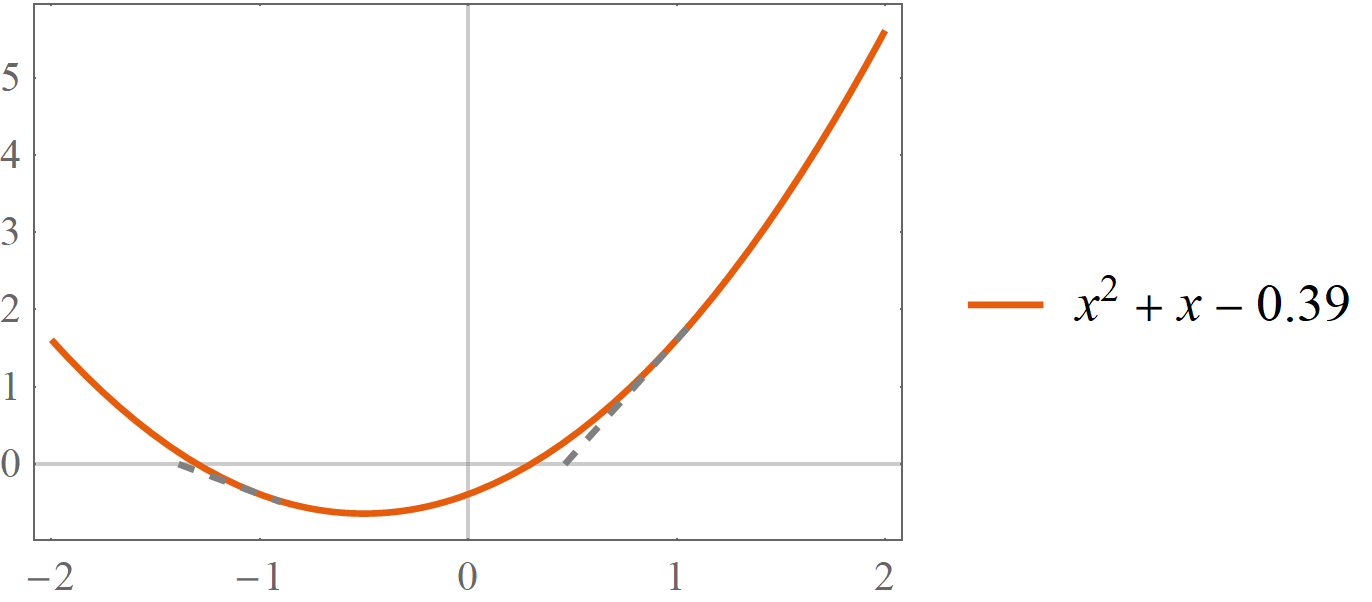
\includegraphics[width=30em]{plot5.png}
  \caption{Newton法}
  \label{fig:plot4}
\end{figure}

Newton法通常比之前的两个线性收敛方法更快:

\begin{table}[htpb]
\centering
\caption{Newton法迭代过程}
$\begin{array}{ccccc}
    \toprule
n & x_n & x_{n+1} & x'_n & x'_{n+1} \\
\midrule
 1 & 1.0000000 & 0.4633333 & -1.0000000 & -1.3900000 \\
 2 & 0.4633333 & 0.3138466 & -1.3900000 & -1.3045506 \\
 3 & 0.3138466 & 0.3001178 & -1.3045506 & -1.3000129 \\
 4 & 0.3001178 & 0.3000000 & -1.3000129 & -1.3000000 \\
 5 & 0.3000000 & 0.3000000 & -1.3000000 & -1.3000000 \\
    \bottomrule
\end{array}\label{table:newton}$
\end{table}

仅用了5步收敛到方程的解。

\section{重根的情况}
对于多重根的情况,Newton法是线性收敛的。

以函数$f(x) = 2\mathrm{e}^{x-1} - x^2 - 1$为例,其$x=1$的根为三重根。

\begin{figure}[htbp]
  \centering
  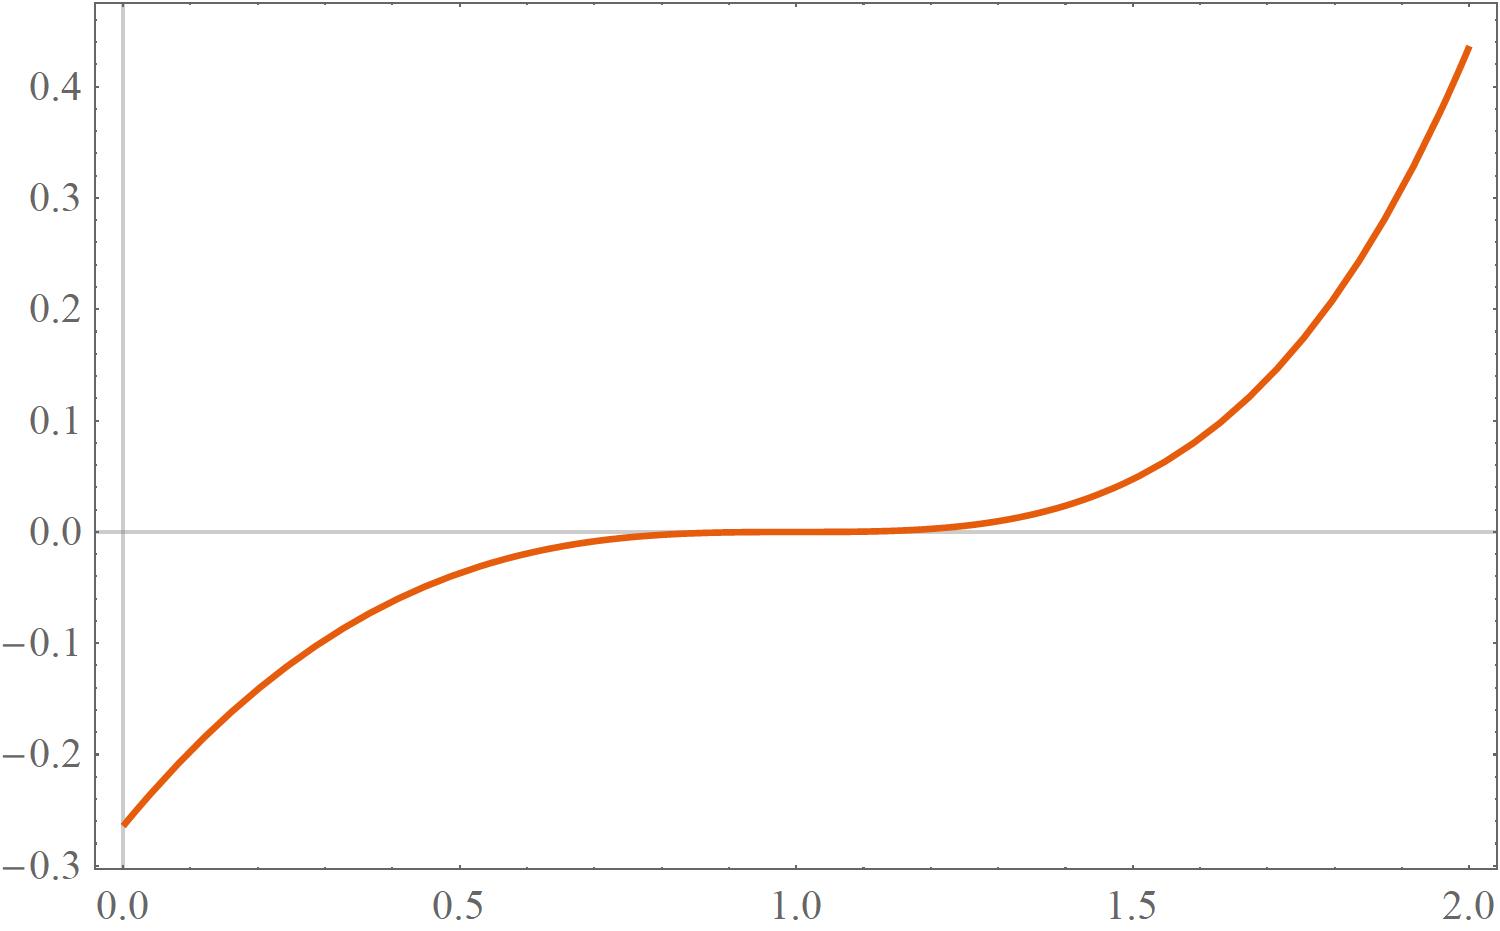
\includegraphics[width=20em]{plot6.png}
  \caption{$f(x) = 2\mathrm{e}^{x-1} - x^2 - 1$}
  \label{fig:plot6}
\end{figure}
\[
f(x) = 2\mathrm{e}^{x-1} - x^2 - 1
\]
\[
f'(x) = 2\mathrm{e}^{x-1} - 2x
\]
\[
f''(x) = 2\mathrm{e}^{x-1} - 2
\]
\[
f'''(x) = 2\mathrm{e}^{x-1}
\]

$f(x)$、$f'(x)$、$f''(x)$在$x=1$处均为零,$f'''(1)=2\neq0$,因此是三重根。

先测试二分法与牛顿法。

二分法的初始区间宽度为$1$($[0.6,1.6]$),精度要求与之前相同,因此设定为20步。得到的输出结果为$1.0000239$,实际上并没有达到我们要求的精度。主要原因是在根附近的函数相当平缓,因此数值误差的影响很大。

而对于Newton法,由于这是一个三重根的情况,$m=3$。所以可以估计其线性收敛速度为$2/3$。以下为其前5步:

\begin{table}[htpb]
\centering
\caption{Newton法迭代过程}
$\begin{array}{ccccc}
    \toprule
n & x_n & e_i/e_{i-1} \\
\midrule
 1 & 1.34049846677307 &  \\
 2 & 1.23029037451719 & 0.676333073389934 \\
 3 & 1.15502223254582 & 0.673159843831200 \\
 4 & 1.10402251421791 & 0.671016747144078 \\
 5 & 1.06965098327047 & 0.669576041245875 \\
\bottomrule
\end{array}\label{table:newton2}$
\end{table}

最终经过30步迭代,得到的解为$1.0000010$。

作为对比,还使用割线法与改进的Newton法进行计算。作为对比,将各方法的收敛情况作图:

\begin{figure}[htbp]
  \centering
  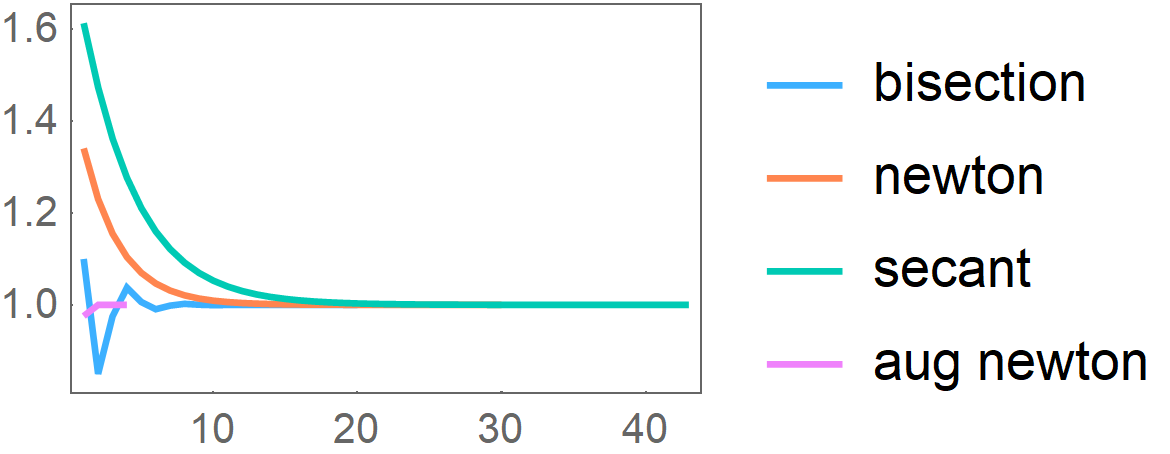
\includegraphics[width=30em]{plot7.png}
  \caption{四种方法收敛情况}
  \label{fig:plot7}
\end{figure}

其中改进Newton法使用的迭代公式如下:
\[
x_{i+1} = x_i - \frac{f(x_i)f'(x_i)}{[f'(x_i)]^2-f(x_i)f''(x_i)}
\]

\end{document}